\section{Implementation}

In this section we describe an implementation of the method described in
section \ref{label{sec:method}} suitable for rapid gravitational-wave searches
for compact binary coalescence.  The previous method requires several
computations that can be done before the analysis is actually underway.  Thus
we divide the procedure into two stages 1) an offline planning stage and 2) an
online, low latency filtering stage.  The offline stage can be done before the
analysis is started an updated asychronously whereas the online stage must keep
up with the detector output and produce search results as rapidly as possible.
In the next two subsections we describe what these stages entail.

\subsection{Planning stage}

The planning stage proceeds as follows.  First, the templates are chosen by
covering the space of mass parameters with a hexagonal grid
\cite{PhysRevD.76.102004} in order to satisfy the minimum match criterion.
Next, the templates are subdivided into groups of neighbors called
``sub-banks'' that are appropriately sized so that each bank can be efficiently
handled by a single machine.  (In this paper, we will only study a single
sub-bank.)  Using our understanding of the time-frequency evolution of the
templates, we choose time slice boundaries such that all of the templates
within this sub-bank are sub-critically sampled at progressively lower sample
rates.  Next, the templates within this sub-bank are realized as \textsc{fir}
filter coefficients.  For each time slice, the templates are downsampled to the
appropriate sample rate.  Finally, the \textsc{svd} is applied to each time
slice in order to produce a set of orthogonal \textsc{fir} filters and a
reconstruction matrix that maps them back to the original templates.  The
downsampled orthogonal \textsc{fir} filter coefficients, the reconstruction
matrix, and the time slice boundaries are all saved to disk.

\subsection{Filtering stage}

We have implemented a prototype of the low latency filtering stage using an
open source signal processing environment called GStreamer \cite{gstreamer}.
GStreamer is a vital component of many Linux systems, providing media playback,
authoring, and streaming on devices from cell phones to desktop computers to
streaming media servers.  It turns out that it is also uniquely suited to
gravitational wave data analysis.  In our application, GStreamer excels at
queueing, synchronizing, adding, and bookkeeping many different signals at
different sample rates.  It also provides some useful signal processing
primitives such as decimators, \textsc{fir} filters, and interpolators.  Most
importantly, it permits us to recruit all of the host system's \textsc{cpu}s
without having to write complicated and error-prone multithreaded code.

\begin{figure}[htbp]
	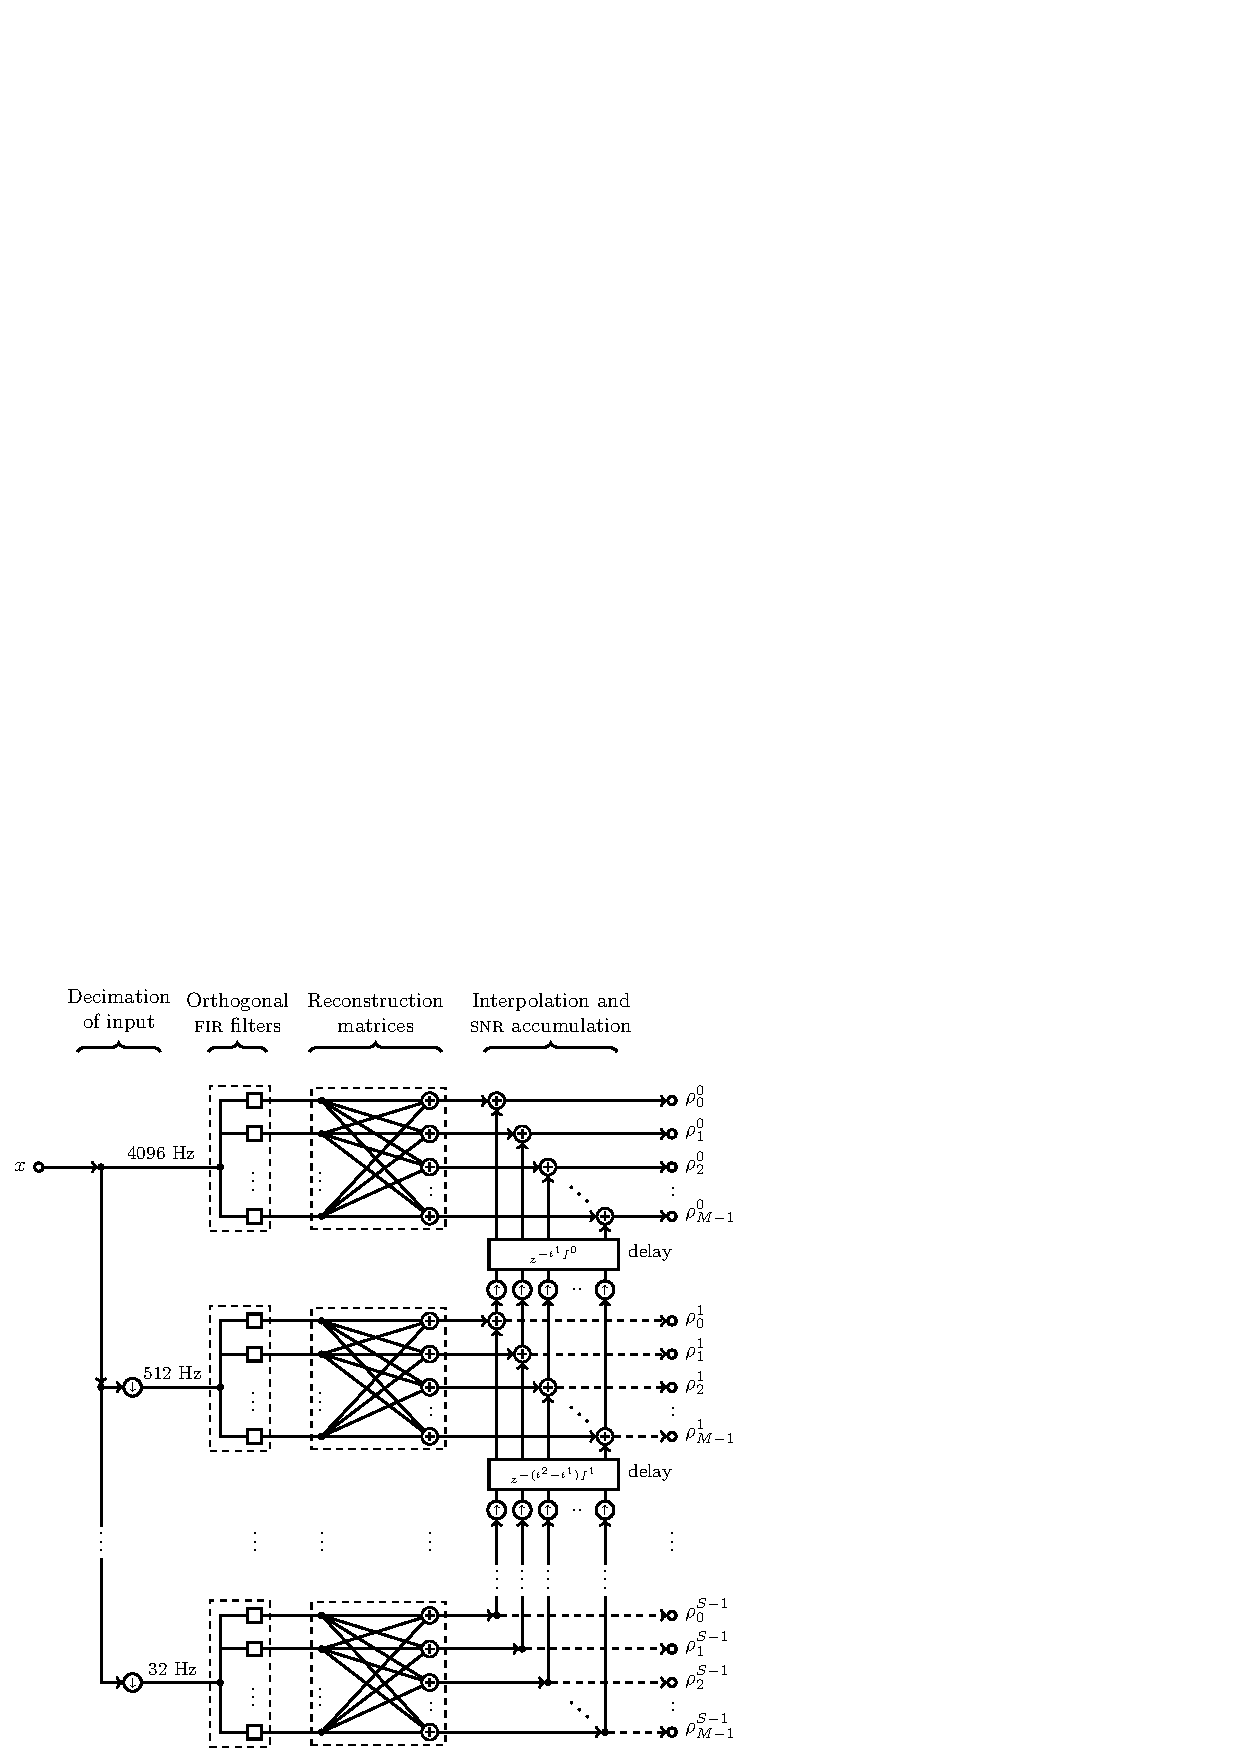
\includegraphics{figures/lloid-diagram.pdf}
	\caption{Schematic of LLOID pipeline illustrating signal flow.  Circles with arrows represent upsampling \protect\includegraphics{figures/upsample-symbol.pdf} or downsampling \protect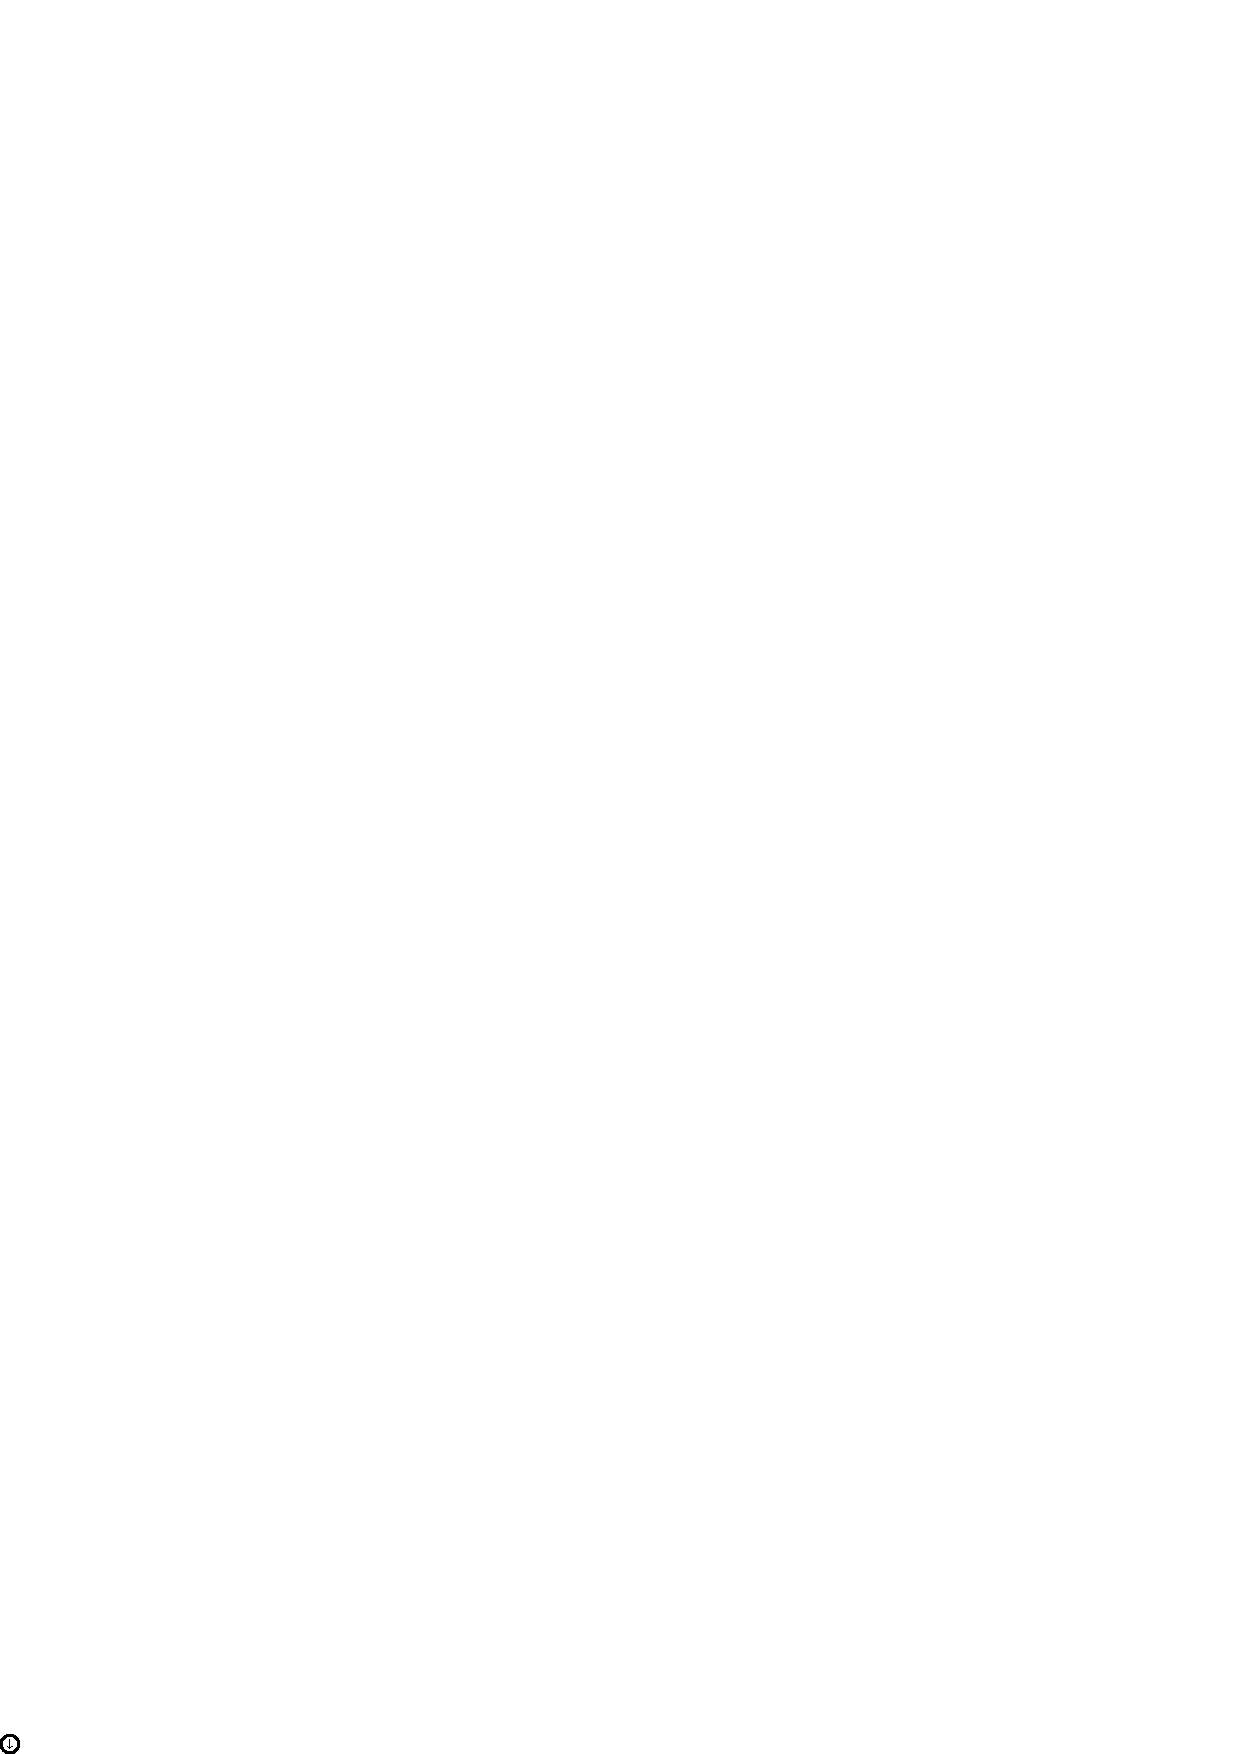
\includegraphics{figures/downsample-symbol.pdf}.  Circles with plus signs represent summing junctions \protect\includegraphics{figures/adder-symbol.pdf}.  Squares \protect\includegraphics{figures/fir-symbol.pdf} stand for FIR filters.  Sample rate decreases from the top of the diagram to the bottom.}
\end{figure}

The filter pipeline consists of six distinct stages.

\subsubsection{Decimation}

First, the sample rate of the whitened detector data is reduced to successively
lower sample rates by decimation.  Decimation involves applying an antialiasing
filter to the data, and then downsampling by deleting samples.  We use a
192-tap \textsc{fir} decimator provided by GStreamer.

\subsubsection{Time delays}

Each decimated detector data stream becomes the input for one time slice, but
it must be appropriately delayed.

\subsubsection{Orthogonal \textsc{fir} filters}

\subsubsection{Reconstruction}

\subsubsection{Interpolation}

\subsubsection{SNR accumulation}

%Our new method consists of six distinct stages:
%\begin{enumerate}
%\item\label{item:decimation} Decimation of the detector data to successively lower sample rates
%\item\label{item:delay} Delay lines to appropriately synchronize of all of the time slices
%\item\label{item:ortho} Application of orthogonal \textsc{fir} filters to the decimated detector data
%\item\label{item:reconstruct} Mixing of orthogonal filter output using reconstruction matrices
%\item\label{item:interpolation} Interpolation of reconstructed output to a common sample rate
%\item\label{item:accumulation} Accumulation of \textsc{snr} from each time slice
%\end{enumerate}
